\documentclass[tikz,border=0pt]{standalone}
\usepackage{xcolor}
\usetikzlibrary{calc}
% Palette: Sam_Comm_final.png by eye, and the drones and raiders.
\definecolor{ink}{HTML}{3B2340}
\definecolor{sky}{HTML}{EFC46A}
\definecolor{skyhi}{HTML}{F5DA92}
\definecolor{skylow}{HTML}{E9B060}
\definecolor{cloud}{HTML}{F2D58A}
\definecolor{paper}{HTML}{FBEFD0}
\definecolor{cream}{HTML}{FFF6E0}
\definecolor{white}{HTML}{FFFFFF}
\definecolor{wallA}{HTML}{E88A73}
\definecolor{wallB}{HTML}{EE9F7E}
\definecolor{wallC}{HTML}{E47A7E}
\definecolor{wallD}{HTML}{F0B07E}
\definecolor{wallE}{HTML}{D9765F}
\definecolor{wallF}{HTML}{E99A8A}
\definecolor{greenA}{HTML}{8DBB7E}
\definecolor{greenB}{HTML}{6FA77A}
\definecolor{greenC}{HTML}{A9C97F}
\definecolor{greenD}{HTML}{5E9C6A}
\definecolor{greenE}{HTML}{4A8060}
\definecolor{sage}{HTML}{9DB98A}
\definecolor{sagedark}{HTML}{6F8F66}
\definecolor{sagelight}{HTML}{C2D6A6}
\definecolor{window}{HTML}{F6E7A0}
\definecolor{windark}{HTML}{8C5A64}
\definecolor{metal}{HTML}{8D9A93}
\definecolor{metaldark}{HTML}{5E6B66}
\definecolor{metallight}{HTML}{B9C4BC}
\definecolor{wood}{HTML}{B9835A}
\definecolor{wooddark}{HTML}{8C5A3C}
\definecolor{woodlight}{HTML}{D9A66F}
\definecolor{stone}{HTML}{E7C9A0}
\definecolor{stonedark}{HTML}{C9A47E}
\definecolor{concrete}{HTML}{D8C3A4}
\definecolor{concretedark}{HTML}{B8A084}
\definecolor{asphalt}{HTML}{8E7A86}
\definecolor{asphaltdark}{HTML}{6E5C68}
\definecolor{roadline}{HTML}{F6E7A0}
\definecolor{kerb}{HTML}{D8B48C}
\definecolor{red}{HTML}{E0483E}
\definecolor{redlight}{HTML}{F27A6A}
\definecolor{gold}{HTML}{FFB000}
\definecolor{goldlight}{HTML}{FFD54F}
\definecolor{teal}{HTML}{4FA3A0}
\definecolor{tealdark}{HTML}{3C8582}
\definecolor{magenta}{HTML}{FF2E88}
\definecolor{cyan}{HTML}{13CFE3}
\definecolor{violet}{HTML}{8A5BD6}
\definecolor{orange}{HTML}{F2803A}
\definecolor{pink}{HTML}{F48FB1}
\definecolor{glow}{HTML}{4FE6E0}
\definecolor{glowhi}{HTML}{C8FFF9}
\definecolor{hot}{HTML}{FF6A1A}
\definecolor{hothi}{HTML}{FFD07A}
\definecolor{armour}{HTML}{7E7A86}
\definecolor{armourdark}{HTML}{5A5466}
\definecolor{armourlight}{HTML}{A8A2B0}
\definecolor{wasp}{HTML}{E0A82E}
\definecolor{waspdark}{HTML}{B07E1A}
\definecolor{moth}{HTML}{F2E6C8}
\definecolor{mothdark}{HTML}{D2C09A}
\definecolor{hornet}{HTML}{3C8582}
\definecolor{hornetdark}{HTML}{2C6260}
\definecolor{warden}{HTML}{E47A7E}
\definecolor{wardendark}{HTML}{B85A62}
\definecolor{tick}{HTML}{8DBB7E}
\definecolor{tickdark}{HTML}{5E8A5A}
\definecolor{strider}{HTML}{D9765F}
\definecolor{striderdark}{HTML}{A8543F}
\definecolor{queen}{HTML}{7E5C94}
\definecolor{queendark}{HTML}{4C3A60}
\definecolor{jacket}{HTML}{6FA77A}
\definecolor{jacketb}{HTML}{4FA3A0}
\definecolor{jacketc}{HTML}{E88A73}
\definecolor{jacketd}{HTML}{F0B07E}
\definecolor{skin}{HTML}{F2C49A}
\definecolor{skinb}{HTML}{C98C6A}
\definecolor{skinc}{HTML}{8C5A3C}
\definecolor{hair}{HTML}{3B2340}
\definecolor{goo}{HTML}{B6E35A}
\definecolor{goodark}{HTML}{7FB23A}
\newcommand{\Ink}{1.15pt}
\tikzset{inked/.style={draw=ink, line width=\Ink, line join=round, line cap=round}}
\begin{document}
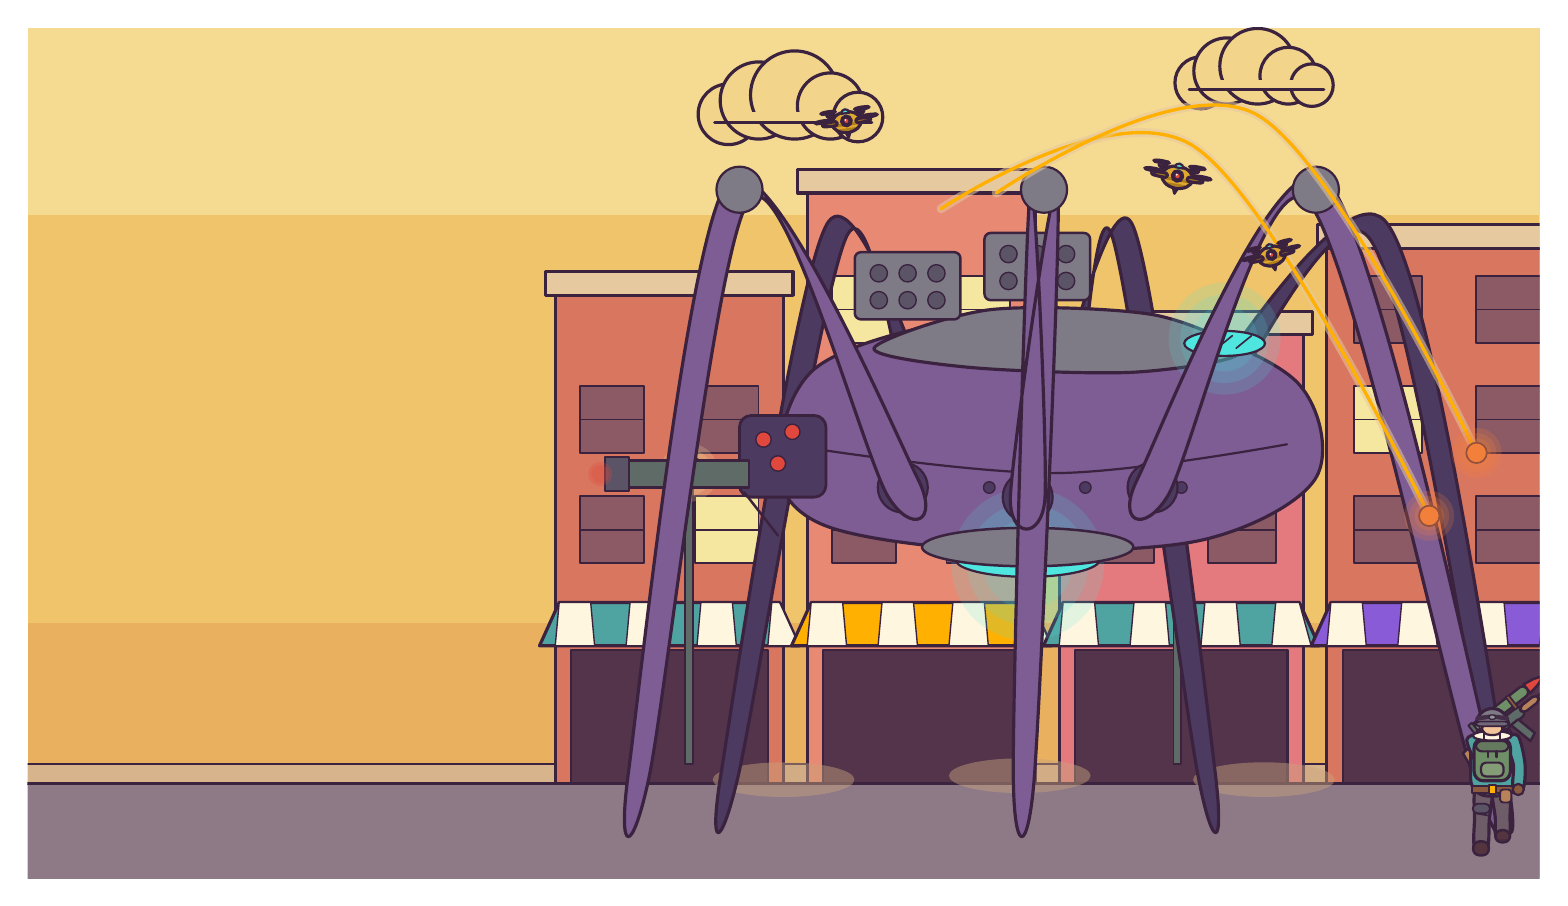
\begin{tikzpicture}
\clip (0,0) rectangle (19.2,10.8);
\fill[sky] (0,0) rectangle (19.2,10.8);
\fill[skyhi] (0,8.424) rectangle (19.2,10.8);
\fill[skylow] (0,0) rectangle (19.2,3.24);
\filldraw[inked,fill=asphalt] (-0.5,-0.5) rectangle (19.7,1.2);
\draw[ink, line width=1pt, line cap=round] (-0.5,1.2) -- (19.7,1.2);
\filldraw[inked,fill=kerb,line width=0.8pt] (-0.5,1.2) rectangle (19.7,1.45);
\begin{scope}\clip (6.4,-1) rectangle (20.2,11.8);
\filldraw[inked,fill=cloud] (8.9,9.7) circle (0.385);
\filldraw[inked,fill=cloud] (9.285,9.875) circle (0.49);
\filldraw[inked,fill=cloud] (9.74,9.945) circle (0.56);
\filldraw[inked,fill=cloud] (10.195,9.805) circle (0.42);
\filldraw[inked,fill=cloud] (10.545,9.665) circle (0.315);
\fill[cloud] (8.9,9.595) rectangle (10.545,9.735);
\draw[ink, line width=1.15pt, line cap=round] (8.725,9.595) -- (10.72,9.595);
\filldraw[inked,fill=cloud] (14.9,10.1) circle (0.33);
\filldraw[inked,fill=cloud] (15.23,10.25) circle (0.42);
\filldraw[inked,fill=cloud] (15.62,10.31) circle (0.48);
\filldraw[inked,fill=cloud] (16.01,10.19) circle (0.36);
\filldraw[inked,fill=cloud] (16.31,10.07) circle (0.27);
\fill[cloud] (14.9,10.01) rectangle (16.31,10.13);
\draw[ink, line width=1.15pt, line cap=round] (14.75,10.01) -- (16.46,10.01);
\filldraw[inked,fill=wallE] (6.7,1.2) rectangle (9.6,7.4);
\filldraw[inked,fill=stone] (6.58,7.4) rectangle (9.72,7.7);
\filldraw[inked,fill=windark,line width=0.7pt] (7.019,4) rectangle (7.831,4.85);
\draw[ink, line width=0.5pt, line cap=round] (7.019,4.42) -- (7.831,4.42);
\filldraw[inked,fill=window,line width=0.7pt] (8.469,4) rectangle (9.281,4.85);
\draw[ink, line width=0.5pt, line cap=round] (8.469,4.42) -- (9.281,4.42);
\filldraw[inked,fill=windark,line width=0.7pt] (7.019,5.4) rectangle (7.831,6.25);
\draw[ink, line width=0.5pt, line cap=round] (7.019,5.82) -- (7.831,5.82);
\filldraw[inked,fill=windark,line width=0.7pt] (8.469,5.4) rectangle (9.281,6.25);
\draw[ink, line width=0.5pt, line cap=round] (8.469,5.82) -- (9.281,5.82);
\filldraw[inked,fill=ink!70!windark,line width=0.8pt] (6.9,1.2) rectangle (9.4,2.9);
\filldraw[inked,fill=teal] (6.75,3.5) -- (9.55,3.5) -- (9.8,2.95) -- (6.5,2.95) -- cycle;
\filldraw[inked,fill=cream,line width=0.5pt] (6.75,3.5) -- (7.15,3.5) -- (7.2,2.95) -- (6.7,2.95) -- cycle;
\filldraw[inked,fill=cream,line width=0.5pt] (7.65,3.5) -- (8.05,3.5) -- (8.1,2.95) -- (7.6,2.95) -- cycle;
\filldraw[inked,fill=cream,line width=0.5pt] (8.55,3.5) -- (8.95,3.5) -- (9,2.95) -- (8.5,2.95) -- cycle;
\filldraw[inked,fill=cream,line width=0.5pt] (9.45,3.5) -- (9.55,3.5) -- (9.8,2.95) -- (9.4,2.95) -- cycle;
\filldraw[inked,fill=wallA] (9.9,1.2) rectangle (12.8,8.7);
\filldraw[inked,fill=stone] (9.78,8.7) rectangle (12.92,9);
\filldraw[inked,fill=windark,line width=0.7pt] (10.219,4) rectangle (11.031,4.85);
\draw[ink, line width=0.5pt, line cap=round] (10.219,4.42) -- (11.031,4.42);
\filldraw[inked,fill=windark,line width=0.7pt] (11.669,4) rectangle (12.481,4.85);
\draw[ink, line width=0.5pt, line cap=round] (11.669,4.42) -- (12.481,4.42);
\filldraw[inked,fill=windark,line width=0.7pt] (10.219,5.4) rectangle (11.031,6.25);
\draw[ink, line width=0.5pt, line cap=round] (10.219,5.82) -- (11.031,5.82);
\filldraw[inked,fill=windark,line width=0.7pt] (11.669,5.4) rectangle (12.481,6.25);
\draw[ink, line width=0.5pt, line cap=round] (11.669,5.82) -- (12.481,5.82);
\filldraw[inked,fill=window,line width=0.7pt] (10.219,6.8) rectangle (11.031,7.65);
\draw[ink, line width=0.5pt, line cap=round] (10.219,7.22) -- (11.031,7.22);
\filldraw[inked,fill=window,line width=0.7pt] (11.669,6.8) rectangle (12.481,7.65);
\draw[ink, line width=0.5pt, line cap=round] (11.669,7.22) -- (12.481,7.22);
\filldraw[inked,fill=ink!70!windark,line width=0.8pt] (10.1,1.2) rectangle (12.6,2.9);
\filldraw[inked,fill=gold] (9.95,3.5) -- (12.75,3.5) -- (13,2.95) -- (9.7,2.95) -- cycle;
\filldraw[inked,fill=cream,line width=0.5pt] (9.95,3.5) -- (10.35,3.5) -- (10.4,2.95) -- (9.9,2.95) -- cycle;
\filldraw[inked,fill=cream,line width=0.5pt] (10.85,3.5) -- (11.25,3.5) -- (11.3,2.95) -- (10.8,2.95) -- cycle;
\filldraw[inked,fill=cream,line width=0.5pt] (11.75,3.5) -- (12.15,3.5) -- (12.2,2.95) -- (11.7,2.95) -- cycle;
\filldraw[inked,fill=cream,line width=0.5pt] (12.65,3.5) -- (12.75,3.5) -- (13,2.95) -- (12.6,2.95) -- cycle;
\filldraw[inked,fill=wallC] (13.1,1.2) rectangle (16.2,6.9);
\filldraw[inked,fill=stone] (12.98,6.9) rectangle (16.32,7.2);
\filldraw[inked,fill=windark,line width=0.7pt] (13.441,4) rectangle (14.309,4.85);
\draw[ink, line width=0.5pt, line cap=round] (13.441,4.42) -- (14.309,4.42);
\filldraw[inked,fill=windark,line width=0.7pt] (14.991,4) rectangle (15.859,4.85);
\draw[ink, line width=0.5pt, line cap=round] (14.991,4.42) -- (15.859,4.42);
\filldraw[inked,fill=windark,line width=0.7pt] (13.441,5.4) rectangle (14.309,6.25);
\draw[ink, line width=0.5pt, line cap=round] (13.441,5.82) -- (14.309,5.82);
\filldraw[inked,fill=windark,line width=0.7pt] (14.991,5.4) rectangle (15.859,6.25);
\draw[ink, line width=0.5pt, line cap=round] (14.991,5.82) -- (15.859,5.82);
\filldraw[inked,fill=ink!70!windark,line width=0.8pt] (13.3,1.2) rectangle (16,2.9);
\filldraw[inked,fill=teal] (13.15,3.5) -- (16.15,3.5) -- (16.4,2.95) -- (12.9,2.95) -- cycle;
\filldraw[inked,fill=cream,line width=0.5pt] (13.15,3.5) -- (13.55,3.5) -- (13.6,2.95) -- (13.1,2.95) -- cycle;
\filldraw[inked,fill=cream,line width=0.5pt] (14.05,3.5) -- (14.45,3.5) -- (14.5,2.95) -- (14,2.95) -- cycle;
\filldraw[inked,fill=cream,line width=0.5pt] (14.95,3.5) -- (15.35,3.5) -- (15.4,2.95) -- (14.9,2.95) -- cycle;
\filldraw[inked,fill=cream,line width=0.5pt] (15.85,3.5) -- (16.15,3.5) -- (16.3,2.95) -- (15.8,2.95) -- cycle;
\filldraw[inked,fill=wallE] (16.5,1.2) rectangle (19.6,8);
\filldraw[inked,fill=stone] (16.38,8) rectangle (19.72,8.3);
\filldraw[inked,fill=windark,line width=0.7pt] (16.841,4) rectangle (17.709,4.85);
\draw[ink, line width=0.5pt, line cap=round] (16.841,4.42) -- (17.709,4.42);
\filldraw[inked,fill=windark,line width=0.7pt] (18.391,4) rectangle (19.259,4.85);
\draw[ink, line width=0.5pt, line cap=round] (18.391,4.42) -- (19.259,4.42);
\filldraw[inked,fill=window,line width=0.7pt] (16.841,5.4) rectangle (17.709,6.25);
\draw[ink, line width=0.5pt, line cap=round] (16.841,5.82) -- (17.709,5.82);
\filldraw[inked,fill=windark,line width=0.7pt] (18.391,5.4) rectangle (19.259,6.25);
\draw[ink, line width=0.5pt, line cap=round] (18.391,5.82) -- (19.259,5.82);
\filldraw[inked,fill=windark,line width=0.7pt] (16.841,6.8) rectangle (17.709,7.65);
\draw[ink, line width=0.5pt, line cap=round] (16.841,7.22) -- (17.709,7.22);
\filldraw[inked,fill=windark,line width=0.7pt] (18.391,6.8) rectangle (19.259,7.65);
\draw[ink, line width=0.5pt, line cap=round] (18.391,7.22) -- (19.259,7.22);
\filldraw[inked,fill=ink!70!windark,line width=0.8pt] (16.7,1.2) rectangle (19.4,2.9);
\filldraw[inked,fill=violet] (16.55,3.5) -- (19.55,3.5) -- (19.8,2.95) -- (16.3,2.95) -- cycle;
\filldraw[inked,fill=cream,line width=0.5pt] (16.55,3.5) -- (16.95,3.5) -- (17,2.95) -- (16.5,2.95) -- cycle;
\filldraw[inked,fill=cream,line width=0.5pt] (17.45,3.5) -- (17.85,3.5) -- (17.9,2.95) -- (17.4,2.95) -- cycle;
\filldraw[inked,fill=cream,line width=0.5pt] (18.35,3.5) -- (18.75,3.5) -- (18.8,2.95) -- (18.3,2.95) -- cycle;
\filldraw[inked,fill=cream,line width=0.5pt] (19.25,3.5) -- (19.55,3.5) -- (19.7,2.95) -- (19.2,2.95) -- cycle;
\filldraw[inked,fill=metaldark,line width=0.6pt] (8.35,1.45) rectangle (8.45,5);
\fill[window, opacity=0.2] (8.4,5.15) circle (0.371);
\fill[window, opacity=0.2] (8.4,5.15) circle (0.294);
\fill[window, opacity=0.2] (8.4,5.15) circle (0.217);
\filldraw[inked,fill=window,line width=0.7pt] (8.4,5.15) circle (0.2);
\filldraw[inked,fill=metaldark,line width=0.6pt] (14.55,1.45) rectangle (14.65,5);
\fill[window, opacity=0.2] (14.6,5.15) circle (0.371);
\fill[window, opacity=0.2] (14.6,5.15) circle (0.294);
\fill[window, opacity=0.2] (14.6,5.15) circle (0.217);
\filldraw[inked,fill=window,line width=0.7pt] (14.6,5.15) circle (0.2);
\fill[stonedark, opacity=0.45]  (9.6,1.25) ellipse (0.9 and 0.22);
\fill[stonedark, opacity=0.45]  (12.6,1.3) ellipse (0.9 and 0.22);
\fill[stonedark, opacity=0.45]  (15.7,1.25) ellipse (0.9 and 0.22);
\begin{scope}[shift={(12.7,1.3)}, rotate=0, xscale=1.22, yscale=1.22]
\filldraw[inked,fill=queendark] plot[smooth cycle, tension=0.5] coordinates {(-1.138,3.341) (-1.873,5.637) (-3.017,-0.018) (-3.193,0.018) (-2.077,5.763) (-0.862,3.459)};
\filldraw[inked,fill=queendark] plot[smooth cycle, tension=0.5] coordinates {(0.156,3.341) (1.083,5.751) (1.954,0.014) (1.776,-0.014) (0.867,5.649) (0.444,3.259)};
\filldraw[inked,fill=queendark] plot[smooth cycle, tension=0.5] coordinates {(1.487,3.499) (3.711,5.784) (4.983,0.02) (4.807,-0.02) (3.539,5.616) (1.713,3.301)};
\filldraw[inked,fill=queen] plot[smooth cycle, tension=0.55] coordinates {(-2.6,3.2) (-2.2,4.25) (-0.6,4.75) (1.4,4.7) (2.8,4.1) (3,3.1) (1.8,2.45) (-0.4,2.35) (-2.1,2.6)};
\filldraw[inked,fill=armour] plot[smooth cycle, tension=0.5] coordinates {(-1.6,4.45) (-0.4,4.85) (1.3,4.8) (2.2,4.4) (1.1,4.2) (-0.6,4.25)};
\draw[ink, line width=0.8pt, line cap=round, line join=round] plot[smooth, tension=0.6] coordinates {(-2.2,3.4) (0.3,3.15) (2.7,3.45)};
\filldraw[inked,fill=queendark,line width=0.5pt] (-1.4,3) circle (0.06);
\filldraw[inked,fill=queendark,line width=0.5pt] (-0.4,3) circle (0.06);
\filldraw[inked,fill=queendark,line width=0.5pt] (0.6,3) circle (0.06);
\filldraw[inked,fill=queendark,line width=0.5pt] (1.6,3) circle (0.06);
\fill[glow, opacity=0.16] (2.05,4.55) circle (0.583);
\fill[glow, opacity=0.16] (2.05,4.55) circle (0.462);
\fill[glow, opacity=0.16] (2.05,4.55) circle (0.341);
\filldraw[inked,fill=glow,line width=0.8pt] (2.05,4.5) ellipse (0.42 and 0.13);
\draw[ink, line width=0.6pt, line cap=round] (1.77,4.45) -- (1.93,4.58);
\draw[ink, line width=0.6pt, line cap=round] (1.97,4.45) -- (2.13,4.58);
\draw[ink, line width=0.6pt, line cap=round] (2.17,4.45) -- (2.33,4.58);
\fill[glow, opacity=0.16] (0,2.2) circle (0.795);
\fill[glow, opacity=0.16] (0,2.2) circle (0.63);
\fill[glow, opacity=0.16] (0,2.2) circle (0.465);
\filldraw[inked,fill=glow,line width=0.8pt] (0,2.25) ellipse (0.75 and 0.18);
\filldraw[inked,fill=armour,line width=0.9pt] (0,2.38) ellipse (1.1 and 0.2);
\filldraw[inked,fill=armour,rounded corners=0.08cm,line width=0.9pt] (-1.8,4.75) rectangle (-0.7,5.45);
\filldraw[inked,fill=armourdark,line width=0.5pt] (-1.55,4.95) circle (0.09);
\filldraw[inked,fill=armourdark,line width=0.5pt] (-1.25,4.95) circle (0.09);
\filldraw[inked,fill=armourdark,line width=0.5pt] (-0.95,4.95) circle (0.09);
\filldraw[inked,fill=armourdark,line width=0.5pt] (-1.55,5.23) circle (0.09);
\filldraw[inked,fill=armourdark,line width=0.5pt] (-1.25,5.23) circle (0.09);
\filldraw[inked,fill=armourdark,line width=0.5pt] (-0.95,5.23) circle (0.09);
\filldraw[inked,fill=armour,rounded corners=0.08cm,line width=0.9pt] (-0.45,4.95) rectangle (0.65,5.65);
\filldraw[inked,fill=armourdark,line width=0.5pt] (-0.2,5.15) circle (0.09);
\filldraw[inked,fill=armourdark,line width=0.5pt] (0.1,5.15) circle (0.09);
\filldraw[inked,fill=armourdark,line width=0.5pt] (0.4,5.15) circle (0.09);
\filldraw[inked,fill=armourdark,line width=0.5pt] (-0.2,5.43) circle (0.09);
\filldraw[inked,fill=armourdark,line width=0.5pt] (0.1,5.43) circle (0.09);
\filldraw[inked,fill=armourdark,line width=0.5pt] (0.4,5.43) circle (0.09);
\filldraw[inked,fill=queendark,rounded corners=0.15cm,line width=1pt] (-3,2.9) rectangle (-2.1,3.75);
\filldraw[inked,fill=metaldark,line width=0.9pt] (-4.2,3) rectangle (-2.9,3.28);
\filldraw[inked,fill=armourdark,line width=0.8pt] (-4.4,2.96) rectangle (-4.15,3.32);
\fill[red, opacity=0.25] (-4.45,3.14) circle (0.126);
\fill[red, opacity=0.25] (-4.45,3.14) circle (0.093);
\filldraw[inked,fill=red,line width=0.5pt] (-2.75,3.5) circle (0.08);
\filldraw[inked,fill=red,line width=0.5pt] (-2.45,3.58) circle (0.08);
\filldraw[inked,fill=red,line width=0.5pt] (-2.6,3.25) circle (0.08);
\draw[ink, line width=0.9pt, line cap=round] (-2.6,2.5) -- (-2.95,2.95);
\filldraw[inked,fill=queendark,line width=0.8pt] (-1.3,3) circle (0.26);
\filldraw[inked,fill=queen] plot[smooth cycle, tension=0.5] coordinates {(-1.458,2.913) (-2.893,6.002) (-3.942,-0.019) (-4.158,0.019) (-3.107,6.198) (-1.142,3.087)};
\filldraw[inked,fill=armour,line width=0.8pt] (-3,6.1) circle (0.24);
\filldraw[inked,fill=queendark,line width=0.8pt] (0,2.9) circle (0.26);
\filldraw[inked,fill=queen] plot[smooth cycle, tension=0.5] coordinates {(-0.18,2.91) (0.315,6.098) (0.07,-0.004) (-0.15,0.004) (0.025,6.102) (0.18,2.89)};
\filldraw[inked,fill=armour,line width=0.8pt] (0.17,6.1) circle (0.24);
\filldraw[inked,fill=queendark,line width=0.8pt] (1.3,3) circle (0.26);
\filldraw[inked,fill=queen] plot[smooth cycle, tension=0.5] coordinates {(1.142,3.087) (3.095,6.209) (4.856,0.03) (4.644,-0.03) (2.905,5.991) (1.458,2.913)};
\filldraw[inked,fill=armour,line width=0.8pt] (3,6.1) circle (0.24);
\end{scope}
\draw[stone, line width=3.2pt, line cap=round, line join=round, opacity=0.55] plot[smooth, tension=0.6] coordinates {(11.6,8.5) (14.8,9.3) (17.8,4.6)};
\draw[gold, line width=1.2pt, line cap=round, line join=round] plot[smooth, tension=0.6] coordinates {(11.6,8.5) (14.8,9.3) (17.8,4.6)};
\filldraw[inked,fill=orange,line width=0.6pt] (17.8,4.6) circle (0.13);
\fill[orange, opacity=0.2] (17.8,4.6) circle (0.318);
\fill[orange, opacity=0.2] (17.8,4.6) circle (0.252);
\fill[orange, opacity=0.2] (17.8,4.6) circle (0.186);
\draw[stone, line width=3.2pt, line cap=round, line join=round, opacity=0.55] plot[smooth, tension=0.6] coordinates {(12.3,8.7) (15.6,9.7) (18.4,5.4)};
\draw[gold, line width=1.2pt, line cap=round, line join=round] plot[smooth, tension=0.6] coordinates {(12.3,8.7) (15.6,9.7) (18.4,5.4)};
\filldraw[inked,fill=orange,line width=0.6pt] (18.4,5.4) circle (0.13);
\fill[orange, opacity=0.2] (18.4,5.4) circle (0.318);
\fill[orange, opacity=0.2] (18.4,5.4) circle (0.252);
\fill[orange, opacity=0.2] (18.4,5.4) circle (0.186);
\begin{scope}[shift={(14.6,8.9)}, rotate=-10, xscale=0.32, yscale=0.32]
\filldraw[inked,fill=waspdark] plot[smooth cycle, tension=0.5] coordinates {(-0.022,0.054) (-0.736,0.313) (-0.704,0.407) (0.022,0.186)};
\filldraw[inked,fill=metaldark,line width=0.8pt] (-0.78,0.32) rectangle (-0.66,0.48);
\filldraw[draw=ink, line width=0.8pt, fill=metallight, fill opacity=0.55] (-0.72,0.5) ellipse (0.32 and 0.064);
\draw[ink, line width=1.1pt, line cap=round] (-0.992,0.46) -- (-0.448,0.54);
\filldraw[inked,fill=metaldark,line width=0.64pt] (-0.72,0.5) circle (0.045);
\filldraw[inked,fill=waspdark] plot[smooth cycle, tension=0.5] coordinates {(-0.022,0.186) (0.704,0.407) (0.736,0.313) (0.022,0.054)};
\filldraw[inked,fill=metaldark,line width=0.8pt] (0.66,0.32) rectangle (0.78,0.48);
\filldraw[draw=ink, line width=0.8pt, fill=metallight, fill opacity=0.55] (0.72,0.5) ellipse (0.32 and 0.064);
\draw[ink, line width=1.1pt, line cap=round] (0.448,0.46) -- (0.992,0.54);
\filldraw[inked,fill=metaldark,line width=0.64pt] (0.72,0.5) circle (0.045);
\filldraw[inked,fill=waspdark,line width=0.9pt] (-0.13,-0.36) -- (0.13,-0.36) -- (0,-0.66) -- cycle;
\fill[wasp]  (0,0) ellipse (0.62 and 0.44);
\begin{scope}\clip  (0,0) ellipse (0.62 and 0.44);
\fill[waspdark] (-0.7,-0.16) rectangle (0.7,-0.04);
\fill[waspdark] (-0.7,-0.36) rectangle (0.7,-0.26);
\end{scope}
\draw[inked]  (0,0) ellipse (0.62 and 0.44);
\fill[glow, opacity=0.2] (0,0.42) circle (0.21);
\fill[glow, opacity=0.2] (0,0.42) circle (0.155);
\filldraw[inked,fill=glow,line width=0.8pt] (-0.17,0.38) arc[start angle=180,end angle=0,radius=0.17] -- cycle;
\filldraw[inked,fill=waspdark] plot[smooth cycle, tension=0.5] coordinates {(-0.45,-0.08) (-0.98,-0.06) (-0.98,0.06) (-0.45,0.08)};
\filldraw[inked,fill=metaldark,line width=0.8pt] (-1.04,-0.04) rectangle (-0.92,0.12);
\filldraw[draw=ink, line width=0.8pt, fill=metallight, fill opacity=0.55] (-0.98,0.14) ellipse (0.36 and 0.072);
\draw[ink, line width=1.1pt, line cap=round] (-1.286,0.1) -- (-0.674,0.18);
\filldraw[inked,fill=metaldark,line width=0.64pt] (-0.98,0.14) circle (0.045);
\filldraw[inked,fill=waspdark] plot[smooth cycle, tension=0.5] coordinates {(0.45,0.08) (0.98,0.06) (0.98,-0.06) (0.45,-0.08)};
\filldraw[inked,fill=metaldark,line width=0.8pt] (0.92,-0.04) rectangle (1.04,0.12);
\filldraw[draw=ink, line width=0.8pt, fill=metallight, fill opacity=0.55] (0.98,0.14) ellipse (0.36 and 0.072);
\draw[ink, line width=1.1pt, line cap=round] (0.674,0.1) -- (1.286,0.18);
\filldraw[inked,fill=metaldark,line width=0.64pt] (0.98,0.14) circle (0.045);
\filldraw[inked,fill=armourdark,line width=0.9pt] (0,0.05) circle (0.22);
\filldraw[inked,fill=red,line width=0.8pt] (0,0.05) circle (0.14);
\fill[white, opacity=0.9] (-0.04,0.1) circle (0.045);
\end{scope}
\begin{scope}[shift={(15.8,7.9)}, rotate=14, xscale=0.28, yscale=0.28]
\filldraw[inked,fill=waspdark] plot[smooth cycle, tension=0.5] coordinates {(-0.022,0.054) (-0.736,0.313) (-0.704,0.407) (0.022,0.186)};
\filldraw[inked,fill=metaldark,line width=0.8pt] (-0.78,0.32) rectangle (-0.66,0.48);
\filldraw[draw=ink, line width=0.8pt, fill=metallight, fill opacity=0.55] (-0.72,0.5) ellipse (0.32 and 0.064);
\draw[ink, line width=1.1pt, line cap=round] (-0.992,0.46) -- (-0.448,0.54);
\filldraw[inked,fill=metaldark,line width=0.64pt] (-0.72,0.5) circle (0.045);
\filldraw[inked,fill=waspdark] plot[smooth cycle, tension=0.5] coordinates {(-0.022,0.186) (0.704,0.407) (0.736,0.313) (0.022,0.054)};
\filldraw[inked,fill=metaldark,line width=0.8pt] (0.66,0.32) rectangle (0.78,0.48);
\filldraw[draw=ink, line width=0.8pt, fill=metallight, fill opacity=0.55] (0.72,0.5) ellipse (0.32 and 0.064);
\draw[ink, line width=1.1pt, line cap=round] (0.448,0.46) -- (0.992,0.54);
\filldraw[inked,fill=metaldark,line width=0.64pt] (0.72,0.5) circle (0.045);
\filldraw[inked,fill=waspdark,line width=0.9pt] (-0.13,-0.36) -- (0.13,-0.36) -- (0,-0.66) -- cycle;
\fill[wasp]  (0,0) ellipse (0.62 and 0.44);
\begin{scope}\clip  (0,0) ellipse (0.62 and 0.44);
\fill[waspdark] (-0.7,-0.16) rectangle (0.7,-0.04);
\fill[waspdark] (-0.7,-0.36) rectangle (0.7,-0.26);
\end{scope}
\draw[inked]  (0,0) ellipse (0.62 and 0.44);
\fill[glow, opacity=0.2] (0,0.42) circle (0.21);
\fill[glow, opacity=0.2] (0,0.42) circle (0.155);
\filldraw[inked,fill=glow,line width=0.8pt] (-0.17,0.38) arc[start angle=180,end angle=0,radius=0.17] -- cycle;
\filldraw[inked,fill=waspdark] plot[smooth cycle, tension=0.5] coordinates {(-0.45,-0.08) (-0.98,-0.06) (-0.98,0.06) (-0.45,0.08)};
\filldraw[inked,fill=metaldark,line width=0.8pt] (-1.04,-0.04) rectangle (-0.92,0.12);
\filldraw[draw=ink, line width=0.8pt, fill=metallight, fill opacity=0.55] (-0.98,0.14) ellipse (0.36 and 0.072);
\draw[ink, line width=1.1pt, line cap=round] (-1.286,0.1) -- (-0.674,0.18);
\filldraw[inked,fill=metaldark,line width=0.64pt] (-0.98,0.14) circle (0.045);
\filldraw[inked,fill=waspdark] plot[smooth cycle, tension=0.5] coordinates {(0.45,0.08) (0.98,0.06) (0.98,-0.06) (0.45,-0.08)};
\filldraw[inked,fill=metaldark,line width=0.8pt] (0.92,-0.04) rectangle (1.04,0.12);
\filldraw[draw=ink, line width=0.8pt, fill=metallight, fill opacity=0.55] (0.98,0.14) ellipse (0.36 and 0.072);
\draw[ink, line width=1.1pt, line cap=round] (0.674,0.1) -- (1.286,0.18);
\filldraw[inked,fill=metaldark,line width=0.64pt] (0.98,0.14) circle (0.045);
\filldraw[inked,fill=armourdark,line width=0.9pt] (0,0.05) circle (0.22);
\filldraw[inked,fill=red,line width=0.8pt] (0,0.05) circle (0.14);
\fill[white, opacity=0.9] (-0.04,0.1) circle (0.045);
\end{scope}
\begin{scope}[shift={(10.4,9.6)}, rotate=8, xscale=0.3, yscale=0.3]
\filldraw[inked,fill=waspdark] plot[smooth cycle, tension=0.5] coordinates {(-0.022,0.054) (-0.736,0.313) (-0.704,0.407) (0.022,0.186)};
\filldraw[inked,fill=metaldark,line width=0.8pt] (-0.78,0.32) rectangle (-0.66,0.48);
\filldraw[draw=ink, line width=0.8pt, fill=metallight, fill opacity=0.55] (-0.72,0.5) ellipse (0.32 and 0.064);
\draw[ink, line width=1.1pt, line cap=round] (-0.992,0.46) -- (-0.448,0.54);
\filldraw[inked,fill=metaldark,line width=0.64pt] (-0.72,0.5) circle (0.045);
\filldraw[inked,fill=waspdark] plot[smooth cycle, tension=0.5] coordinates {(-0.022,0.186) (0.704,0.407) (0.736,0.313) (0.022,0.054)};
\filldraw[inked,fill=metaldark,line width=0.8pt] (0.66,0.32) rectangle (0.78,0.48);
\filldraw[draw=ink, line width=0.8pt, fill=metallight, fill opacity=0.55] (0.72,0.5) ellipse (0.32 and 0.064);
\draw[ink, line width=1.1pt, line cap=round] (0.448,0.46) -- (0.992,0.54);
\filldraw[inked,fill=metaldark,line width=0.64pt] (0.72,0.5) circle (0.045);
\filldraw[inked,fill=waspdark,line width=0.9pt] (-0.13,-0.36) -- (0.13,-0.36) -- (0,-0.66) -- cycle;
\fill[wasp]  (0,0) ellipse (0.62 and 0.44);
\begin{scope}\clip  (0,0) ellipse (0.62 and 0.44);
\fill[waspdark] (-0.7,-0.16) rectangle (0.7,-0.04);
\fill[waspdark] (-0.7,-0.36) rectangle (0.7,-0.26);
\end{scope}
\draw[inked]  (0,0) ellipse (0.62 and 0.44);
\fill[glow, opacity=0.2] (0,0.42) circle (0.21);
\fill[glow, opacity=0.2] (0,0.42) circle (0.155);
\filldraw[inked,fill=glow,line width=0.8pt] (-0.17,0.38) arc[start angle=180,end angle=0,radius=0.17] -- cycle;
\filldraw[inked,fill=waspdark] plot[smooth cycle, tension=0.5] coordinates {(-0.45,-0.08) (-0.98,-0.06) (-0.98,0.06) (-0.45,0.08)};
\filldraw[inked,fill=metaldark,line width=0.8pt] (-1.04,-0.04) rectangle (-0.92,0.12);
\filldraw[draw=ink, line width=0.8pt, fill=metallight, fill opacity=0.55] (-0.98,0.14) ellipse (0.36 and 0.072);
\draw[ink, line width=1.1pt, line cap=round] (-1.286,0.1) -- (-0.674,0.18);
\filldraw[inked,fill=metaldark,line width=0.64pt] (-0.98,0.14) circle (0.045);
\filldraw[inked,fill=waspdark] plot[smooth cycle, tension=0.5] coordinates {(0.45,0.08) (0.98,0.06) (0.98,-0.06) (0.45,-0.08)};
\filldraw[inked,fill=metaldark,line width=0.8pt] (0.92,-0.04) rectangle (1.04,0.12);
\filldraw[draw=ink, line width=0.8pt, fill=metallight, fill opacity=0.55] (0.98,0.14) ellipse (0.36 and 0.072);
\draw[ink, line width=1.1pt, line cap=round] (0.674,0.1) -- (1.286,0.18);
\filldraw[inked,fill=metaldark,line width=0.64pt] (0.98,0.14) circle (0.045);
\filldraw[inked,fill=armourdark,line width=0.9pt] (0,0.05) circle (0.22);
\filldraw[inked,fill=red,line width=0.8pt] (0,0.05) circle (0.14);
\fill[white, opacity=0.9] (-0.04,0.1) circle (0.045);
\end{scope}
\begin{scope}[shift={(18.6,0.3)}, rotate=0, xscale=0.55, yscale=0.55]
\begin{scope}[shift={(0.45,2.55)}, rotate=38, xscale=0.85, yscale=0.85]
\filldraw[inked,fill=wood,line width=0.9pt] (-1.25,0.25) -- (-0.4,0.45) -- (-0.35,0.68) -- (-1.2,0.62) -- cycle;
\filldraw[inked,fill=wooddark,line width=0.9pt] (-0.05,0) -- (0.15,0) -- (0.2,0.42) -- (0,0.42) -- cycle;
\filldraw[inked,fill=metaldark,rounded corners=0.05cm,line width=0.9pt] (-0.45,0.4) rectangle (0.8,0.7);
\filldraw[inked,fill=metaldark,line width=0.9pt] (0.3,0.42) -- (0.55,0.42) -- (0.68,-0.15) -- (0.45,-0.25) -- cycle;
\filldraw[inked,fill=wood,rounded corners=0.06cm,line width=0.9pt] (0.75,0.46) rectangle (1.35,0.66);
\filldraw[inked,fill=metaldark,line width=0.8pt] (1.35,0.52) rectangle (2.15,0.6);
\filldraw[inked,fill=metaldark,line width=0.7pt] (2.1,0.49) rectangle (2.22,0.63);
\filldraw[inked,fill=sagedark,rounded corners=0.06cm,line width=0.9pt] (-0.6,0.78) rectangle (1.25,1.08);
\filldraw[inked,fill=red,line width=0.9pt] (1.25,0.78) -- (1.55,0.83) -- (1.82,0.93) -- (1.55,1.03) -- (1.25,1.08) -- cycle;
\filldraw[inked,fill=metaldark,line width=0.7pt] (-0.62,0.74) rectangle (-0.5,1.12);
\filldraw[inked,fill=wooddark,line width=0.6pt] (-0.1,0.68) rectangle (0,1.1);
\filldraw[inked,fill=wooddark,line width=0.6pt] (0.65,0.68) rectangle (0.75,1.1);
\end{scope}
\filldraw[inked,fill=asphaltdark] plot[smooth cycle, tension=0.5] coordinates {(-0.01,1.489) (-0.07,0.792) (-0.11,0.175) (-0.41,0.185) (-0.41,0.808) (-0.39,1.511)};
\filldraw[inked,fill=asphaltdark] plot[smooth cycle, tension=0.5] coordinates {(0.39,1.512) (0.41,0.856) (0.39,0.42) (0.09,0.42) (0.07,0.844) (0.01,1.488)};
\draw[ink, line width=0.6pt, line cap=round, line join=round] plot[smooth, tension=0.6] coordinates {(-0.38,0.95) (-0.1,0.9)};
\filldraw[inked,fill=armourdark,rounded corners=0.06cm,line width=0.7pt] (-0.45,0.95) rectangle (-0.05,1.17);
\filldraw[inked,fill=ink!70!wooddark,rounded corners=0.08cm,line width=0.9pt] (-0.44,-0.02) rectangle (-0.08,0.3);
\filldraw[inked,fill=ink!70!wooddark,rounded corners=0.08cm,line width=0.9pt] (0.07,0.28) rectangle (0.41,0.56);
\fill[ink, opacity=0.35] (0.1,0.3) rectangle (0.38,0.36);
\filldraw[inked,fill=jacketb,rounded corners=0.22cm] (-0.5,1.35) rectangle (0.5,2.85);
\filldraw[inked,fill=wooddark,line width=0.8pt] (-0.47,1.42) rectangle (0.47,1.58);
\filldraw[inked,fill=gold,line width=0.6pt] (-0.08,1.4) rectangle (0.08,1.6);
\filldraw[inked,fill=wood,rounded corners=0.04cm,line width=0.7pt] (0.18,1.2) rectangle (0.44,1.5);
\filldraw[inked,fill=jacketb] plot[smooth cycle, tension=0.5] coordinates {(0.594,2.741) (0.754,2.117) (0.72,1.546) (0.48,1.554) (0.486,2.083) (0.306,2.659)};
\filldraw[inked,fill=wooddark,line width=0.8pt] (0.6,1.5) circle (0.13);
\filldraw[inked,fill=jacketb] plot[smooth cycle, tension=0.5] coordinates {(-0.311,2.756) (-0.169,2.308) (0.135,2.369) (0.165,2.131) (-0.331,2.092) (-0.589,2.644)};
\filldraw[inked,fill=wooddark,line width=0.8pt] (0.18,2.27) circle (0.13);
\draw[ink, line width=2pt, line cap=round] (-0.32,2.85) -- (-0.3,2.3);
\draw[ink, line width=2pt, line cap=round] (0.32,2.85) -- (0.3,2.3);
\filldraw[inked,fill=sagedark,rounded corners=0.12cm] (-0.42,1.7) rectangle (0.42,2.68);
\filldraw[inked,fill=sagedark!80!ink,rounded corners=0.08cm,line width=0.8pt] (-0.38,2.38) rectangle (0.38,2.62);
\filldraw[inked,fill=sagedark!85!paper,rounded corners=0.06cm,line width=0.8pt] (-0.26,1.8) rectangle (0.26,2.12);
\draw[ink, line width=1pt, line cap=round] (-0.1,2.38) -- (-0.1,2.25);
\draw[ink, line width=1pt, line cap=round] (0.1,2.38) -- (0.1,2.25);
\filldraw[inked,fill=cream,line width=0.8pt] (0,2.74) ellipse (0.45 and 0.11);
\draw[ink, line width=0.7pt, line cap=round] (-0.18,2.63) -- (-0.18,2.85);
\draw[ink, line width=0.7pt, line cap=round] (0.18,2.63) -- (0.18,2.85);
\filldraw[inked,fill=skin,line width=0.6pt] (-0.24,2.97) ellipse (0.06 and 0.09);
\filldraw[inked,fill=skin,line width=0.6pt] (0.24,2.97) ellipse (0.06 and 0.09);
\filldraw[inked,fill=skin,rounded corners=0.1cm,line width=0.8pt] (-0.24,2.76) rectangle (0.24,3.05);
\filldraw[inked,fill=armour] (-0.37,3.0) arc[start angle=180,end angle=0,radius=0.37] -- cycle;
\filldraw[inked,fill=armour!80!ink,rounded corners=0.05cm,line width=0.7pt] (-0.39,2.96) rectangle (0.39,3.07);
\draw[ink!80!asphaltdark, line width=1.6pt, line cap=round, line join=round] plot[smooth, tension=0.6] coordinates {(-0.34,3.14) (0,3.18) (0.34,3.14)};
\filldraw[inked,fill=metal,rounded corners=0.03cm,line width=0.5pt] (-0.08,3.12) rectangle (0.08,3.22);
\end{scope}
\end{scope}
\end{tikzpicture}
\end{document}
